\chapter{Physiological Requirements}
\begin{itemize}
	\item How requirements are different from specifications?
    \item What are the forms of the requirements?
    \item How can the requirements be represented?
    \item Are those requirements binary?
    \item Are those requirements equally important?
\end{itemize}

% \begin{itemize}
% 	\item In contrast to specifications
%     \item Specified on physiological conditions during closed-loop interaction between the patient and the device.
%     \item Timing requirements
%     \item Monitor construction
% \end{itemize}
Physiological requirements for medical devices specify the closed-loop conditions that the devices are designed to achieve with its outputs to the patient. Unlike \emph{specifications} which specify desired device actions in response to the inputs from the patients, physiological requirements focus on the conditions of the patient with and without the device, which would indicate whether the device has fulfilled its intended goals. For example, the most basic goal for a pacemaker is to maintain the ventricular rate above certain level. The corresponding physiological requirement is:

 \emph{The interval between two ventricular contractions should always be less or equal to 1000ms.} 

Note that this requirement focus purely on the condition of the patient (ventricular contractions), and there is no mention of the operation of the pacemaker or how the pacemaker should achieve the requirement. An example specification of a single chamber pacemaker corresponding to the requirement is:  

\emph{The pacemaker should deliver ventricular pacing, if there is no sensed ventricular event 1000ms since the last ventricular event (sensed or paced).}
 
The specification is described using internal terminologies of the pacemaker software (paced and sensed events), and specified the action of the pacemaker corresponding to certain inputs. For more complex requirements, multiple specifications have to work together to achieve the requirement. Therefore there may exist executions that satisfy all the specifications but not the corresponding requirement. Verifying physiological requirements requires knowledge of the physiological condition and how device interacts with the physiological environment, thus can only be performed in closed-loop. 

Devices are designed to improve certain physiological conditions, the performance of the devices is evaluated on the difference between the patient conditions without the device and with the device. The device should also avoid deteriorating certain patient conditions, thus physiological requirements are specified in the form of:
$$C_{pre}\rightarrow C_{post}$$
in which $C_{pre}$ is the physiological conditions without the device,  and $C_{post}$ is the physiological condition with the device. For model-based closed-loop verification, $C_{pre}$ is often in form of a set of constraints on patient parameters. As a special case, $C_{pre}$ can equal to $true$, means that $C_{post}$ should be satisfied under all possible conditions.

One of the challenge for developing medical device software is to convert physiological requirements, generally in forms of descriptions of physiological conditions, into mathematical descriptions that can be used by verification tools.  In model-based verification, these physiological conditions have to be mapped onto constraints on model parameters. %In the following section, we use the heart model as example to show this process.

The devices are supposed to deal with all possible environment conditions. However in certain extreme conditions, not all physiological requirements can be satisfied due to the limitations of device functions. It is thus intuitive to assign priorities to the requirements and assess the capability of the device to prioritize more important requirements in these scenarios. 

In this chapter, we use pacemaker as example to demonstrate how to convert physiological descriptions into mathematical requirements and how priorities of the requirements affect the verification process.

%For convenience, requirements are usually specified with binary results (satisfied/unsatisfied). quantitative

\section{Encoding Physiological Conditions}
\figref{state} list some example heart conditions and their corresponding constraints on heart model parameters.
\begin{figure}[!t]
	\center
%		\vspace{-10pt}
	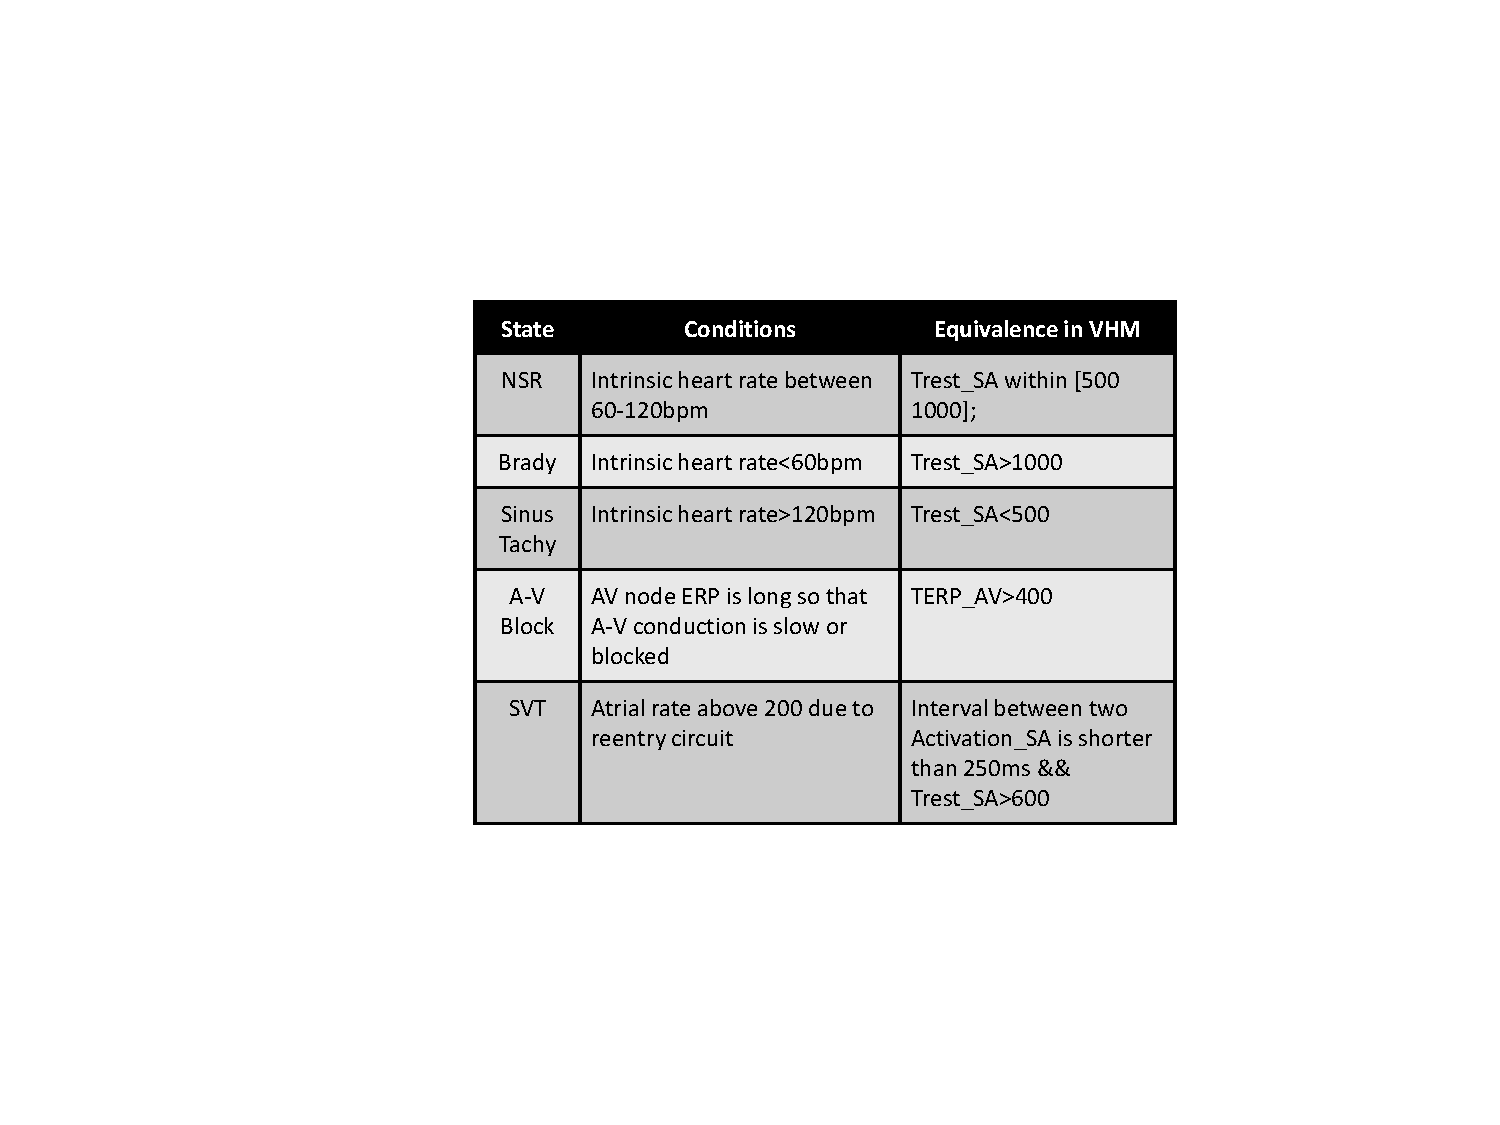
\includegraphics[width=0.70\textwidth]{figs/state.pdf}
	\center
	
	\caption{Patient state and equivalence in VHM}
	\label{fig:state}
\end{figure}
\section{Conditional Requirements}
Physiological requirements are in general conditional requirements. Specifying conditional requirements enables stronger constraints on the closed-loop system. \figref{conditional} shows a list of conditional requirements used during the pacemaker case study. 
\begin{figure}[!b]
	\center
	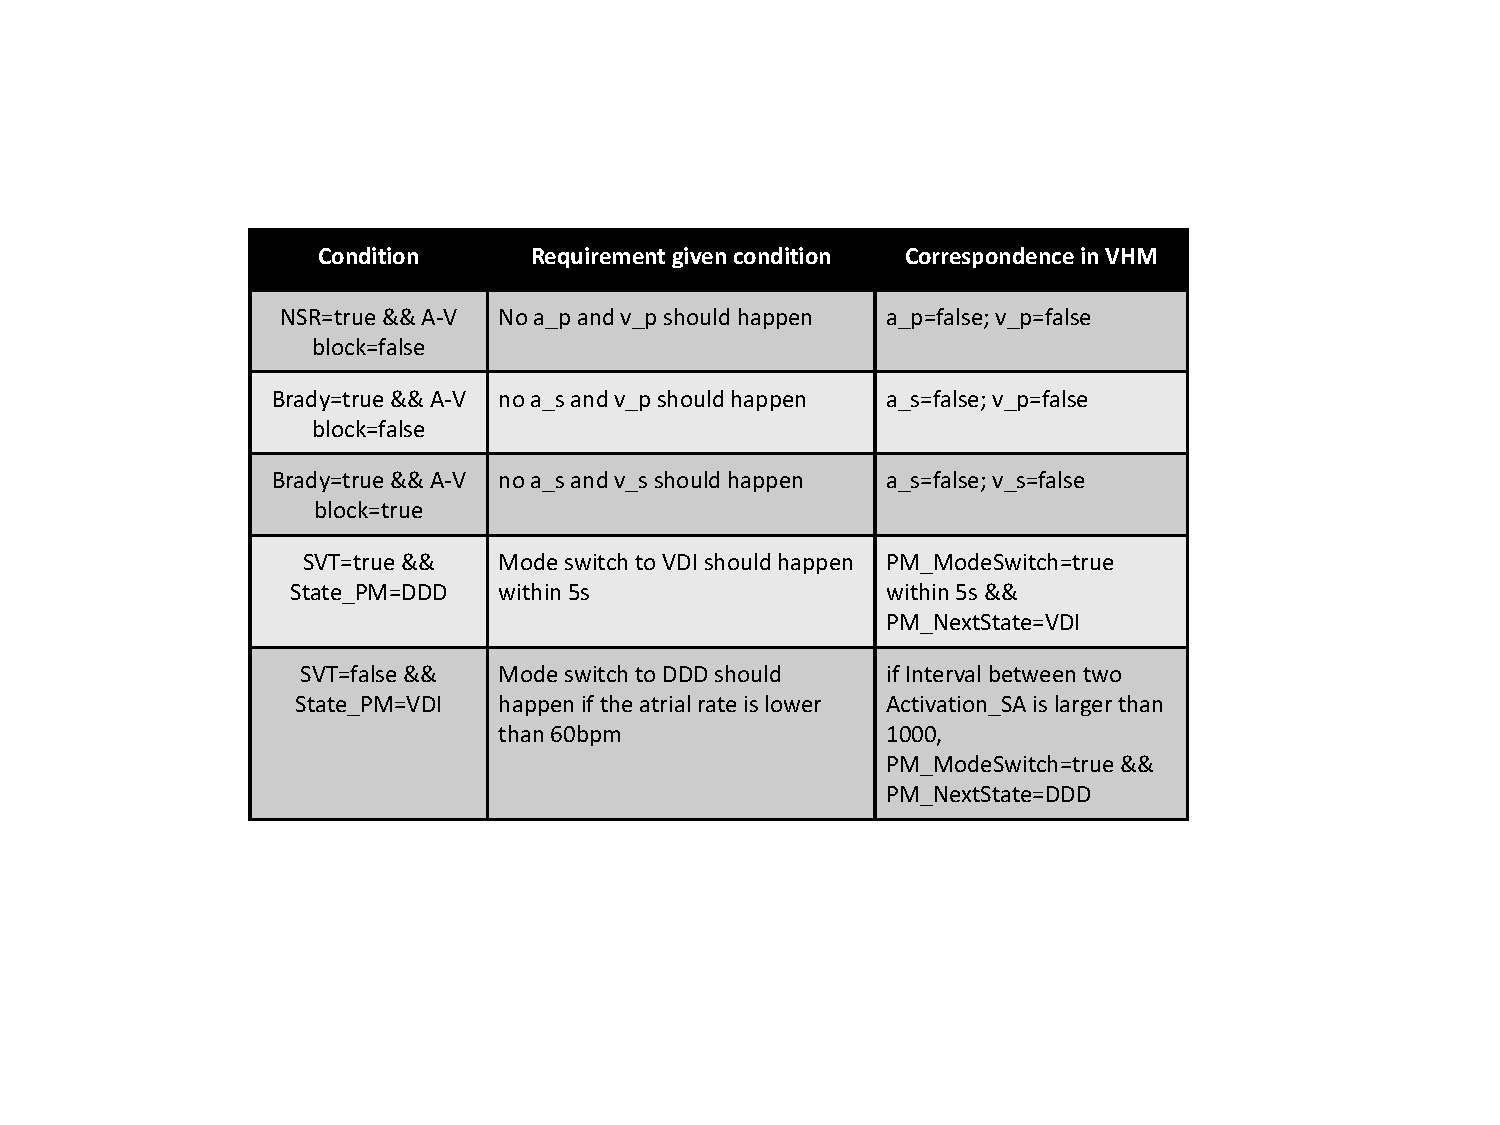
\includegraphics[width=0.8\textwidth]{figs/conditional.pdf}
	\center
	\caption{Conditional requirements for the close-loop system}
		%\vspace{-15pt}
	\label{fig:conditional}
\end{figure}
\section{Requirement Hierarchy}
For a closed-loop system including a heart $H$ and a pacemaker $P$: $S=H || P$ and two requirements $\varphi_1$ and $\varphi_2$ such that $\mathbb{P}_{\varphi_1}<\mathbb{P}_{\varphi_2}$, the following statement should always hold:

$$H\models\varphi_2\rightarrow H||P\models\varphi_2$$
meaning if a higher priority requirement is satisfied by the open-loop environment, it should be satisfied by the closed-loop system as well. An example violation of the statement is:
$$H\not\models\varphi_1 \&\& H\models\varphi_2 \&\& H||P\models\varphi_1 \&\& H||P\not\models\varphi_2$$
which should not be allowed. In our closed-loop verification of pacemaker, the list of physiological requirements with assigned priorities are showing in \figref{properties}.

\begin{figure}[!t]
	\center
	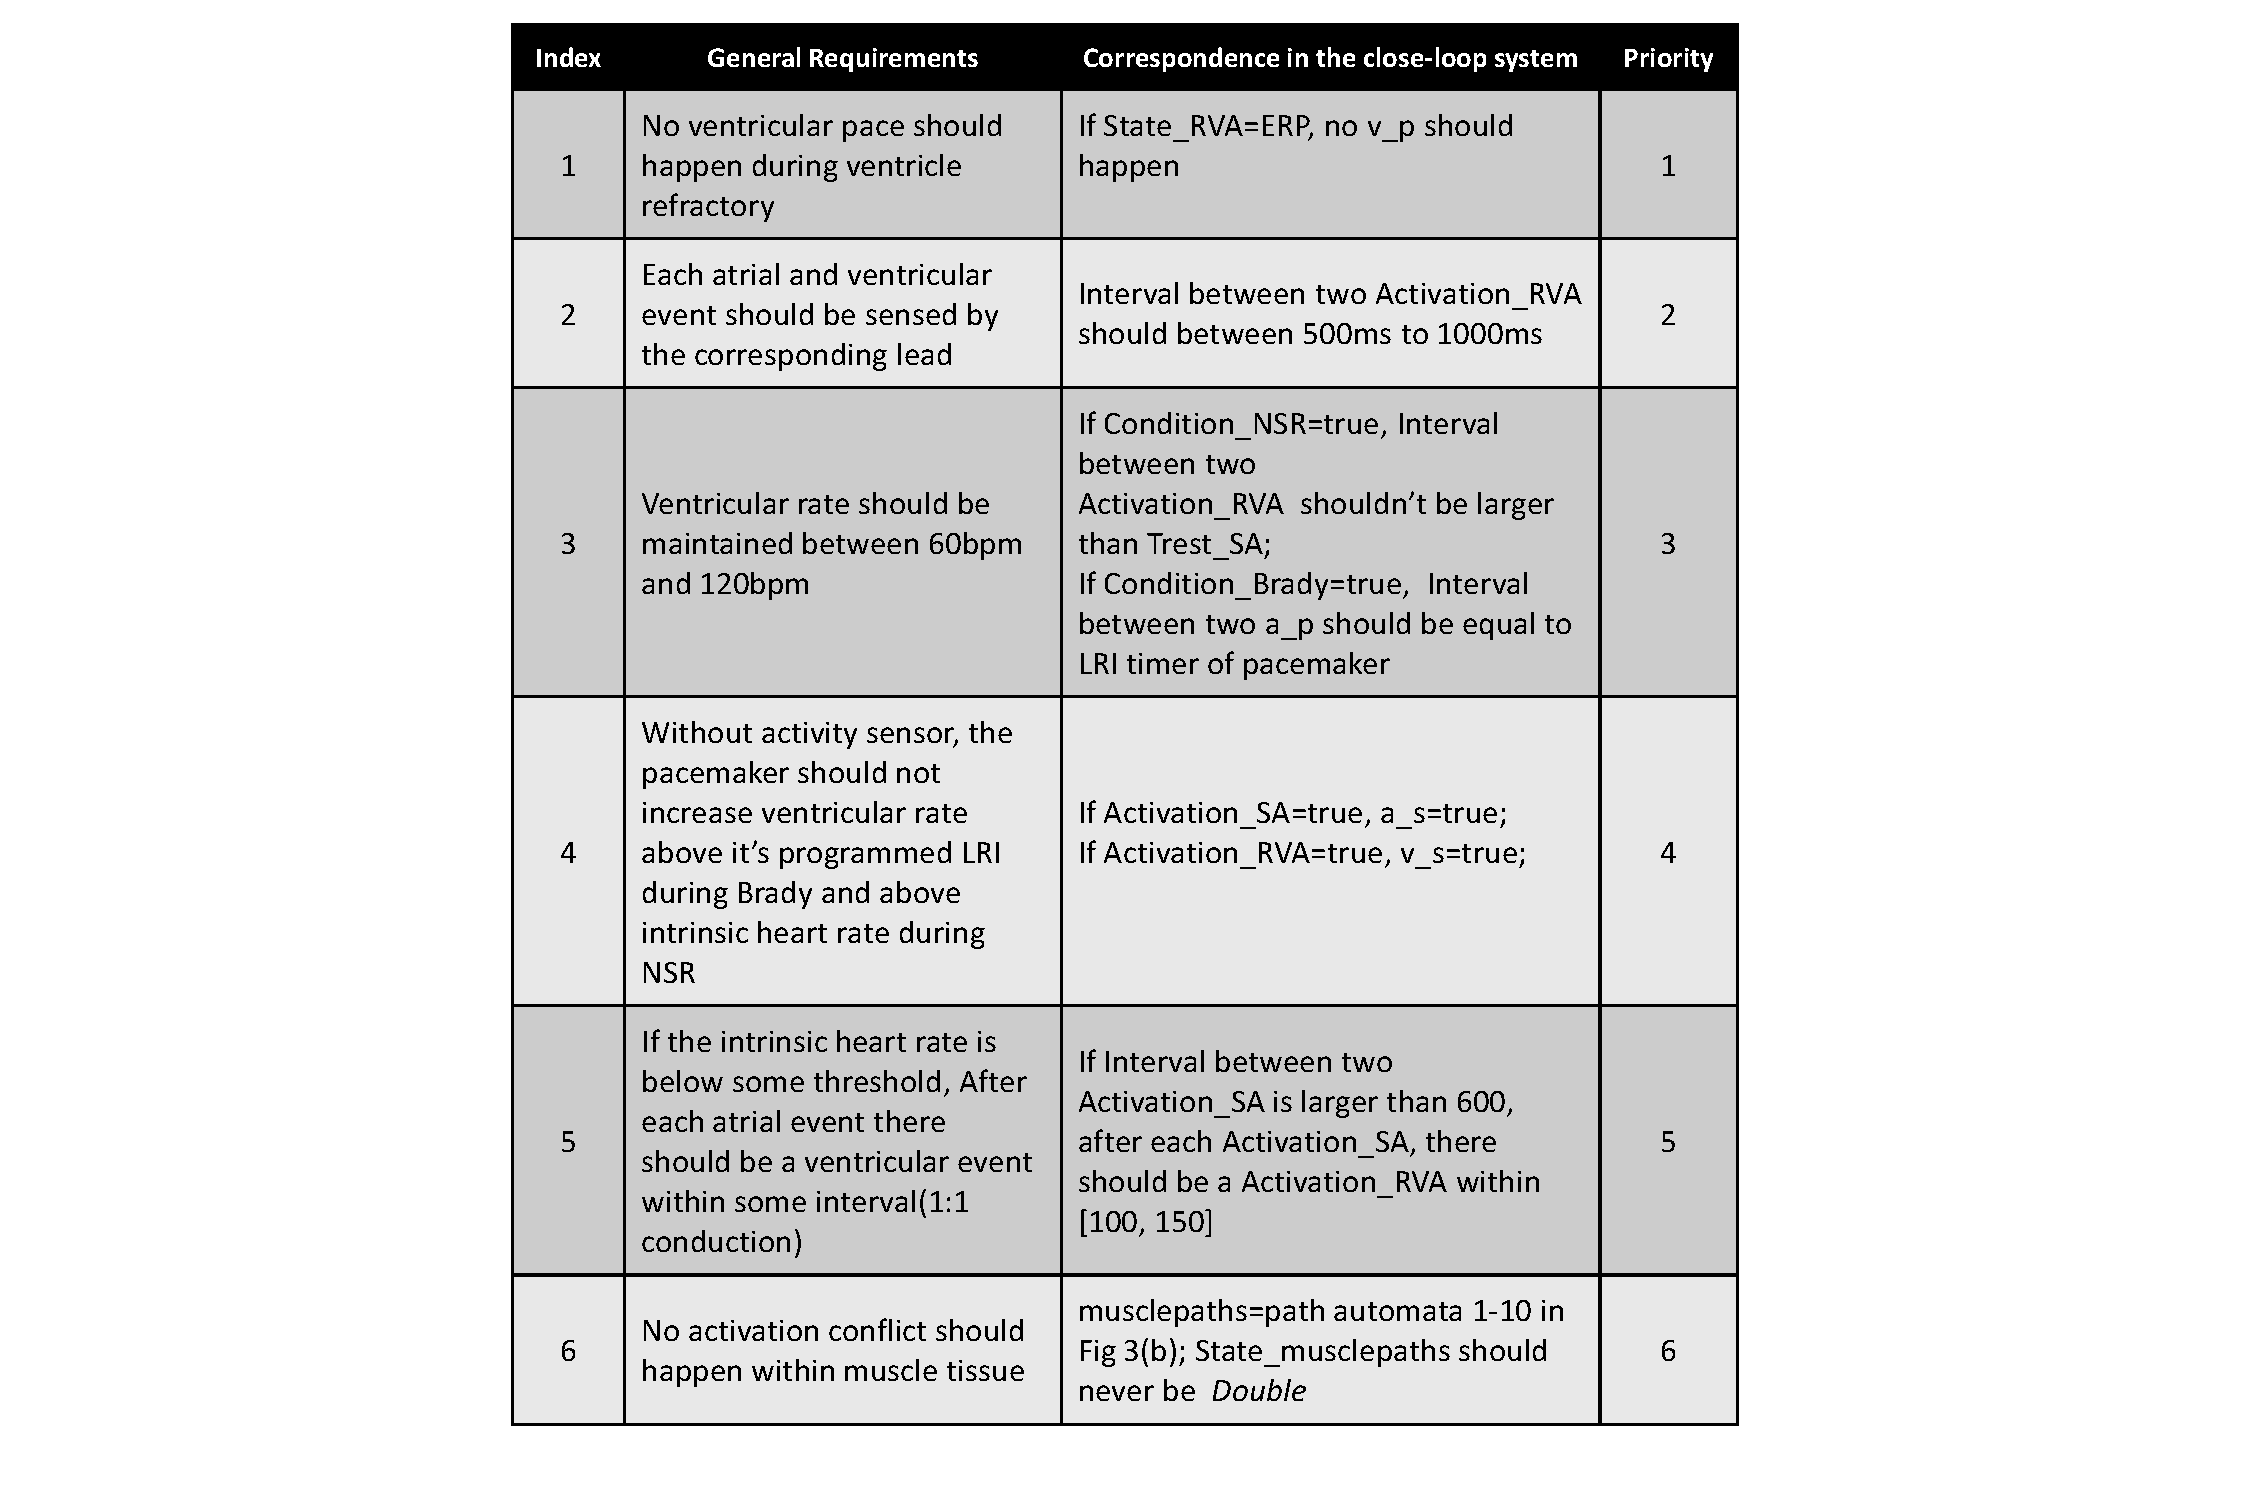
\includegraphics[width=0.7\textwidth]{figs/properties.pdf}
	\center
	\caption{General requirements for the close-loop system}
		%\vspace{-15pt}
	\label{fig:properties}
\end{figure}


%\section{Requirement Representations}
%\subsection{TCTL}
%\subsection{Simulink Block}

